\documentclass[]{article}
\usepackage{amsmath}
\usepackage{amsthm}
\usepackage{listings}
\usepackage[margin=1.3cm]{geometry}
\usepackage{graphicx}
\usepackage{hyperref}
%\usepackage{cleveref} %for the cref command

\title{Practical Lab Numerical Computing Computational Finance \\Bachelor-Worksheet 3}
\author{Lukas Troska, Ilja Kalmykov}
\date{}
\setlength{\parindent}{0pt}

\begin{document}

\maketitle

The source code can be found at \url{https://github.com/iljaGH/CompFin/}.

\section*{Task 2}
See task2.cpp for code.

\section*{Task 3}
Convergence of discrete geometric average option with $S(0)=10,r=0.1,\sigma=0.25,T=1,K=10$ for both $M=10$ and $M=200$ time steps.
As we can see, the number of time steps does not affect the convergence.
\begin{figure}[!ht]
\centering
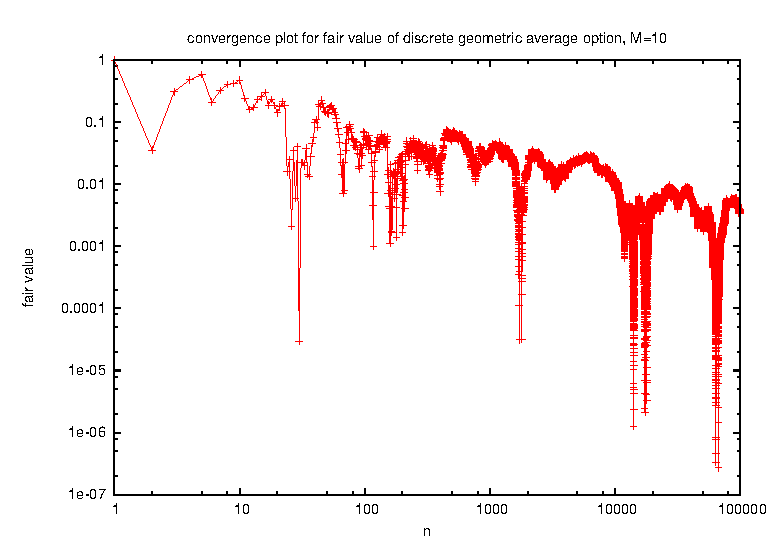
\includegraphics[width=.9\textwidth]{task3_10.eps}
\caption{Convergence plot for the fair value of discrete geometric average
option, $M = 10$.}
\label{fig:Task3a}
\end{figure}
\begin{figure}[!ht]
\centering
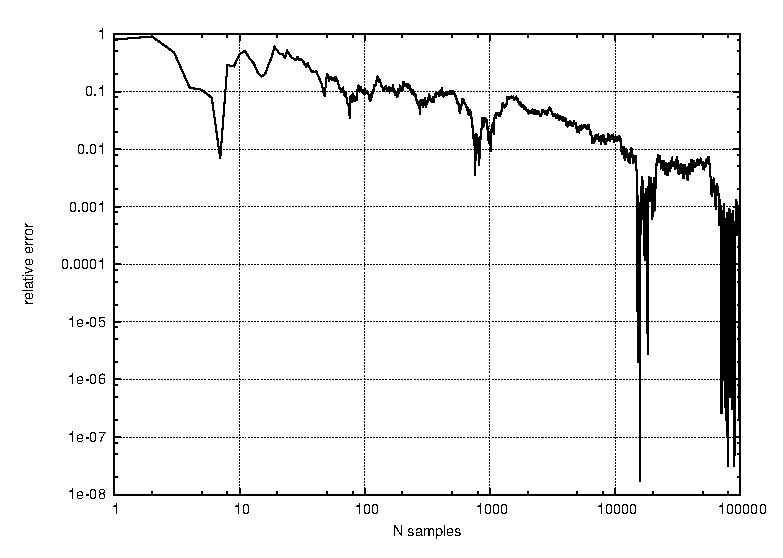
\includegraphics[width=.9\textwidth]{task3_200.eps}
\caption{Convergence plot for the fair value of discrete geometric average
option, $M = 200$.}
\label{fig:Task3b}
\end{figure}
\clearpage

\section*{Task 4} Approximation of continuous geometric average option by discrete geometric average option with $S(0)=10,r=0.1,\sigma=0.25,T=1,K=10$. See task4.cpp for code.
\begin{figure}[!ht]
\centering
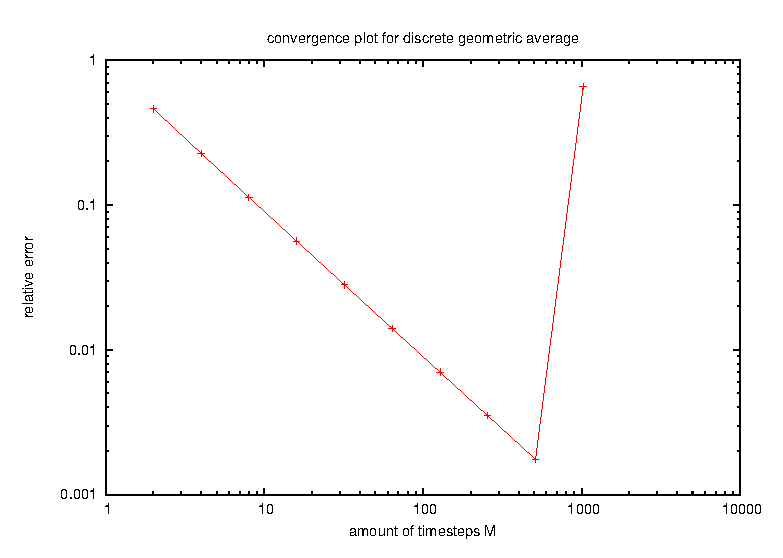
\includegraphics[width=.9\textwidth]{task4.eps}
\caption{Convergence plot for the discrete geometric average option.}
\label{fig:Task4}
\end{figure}
\clearpage

\section*{Task 5} Integrand of the discrete arithmetic average for $M=2,S(0)=10,r=0.1,\sigma=0.25,T=1,K=10$. See task5.cpp for code.\\
\begin{figure}[!ht]
\centering
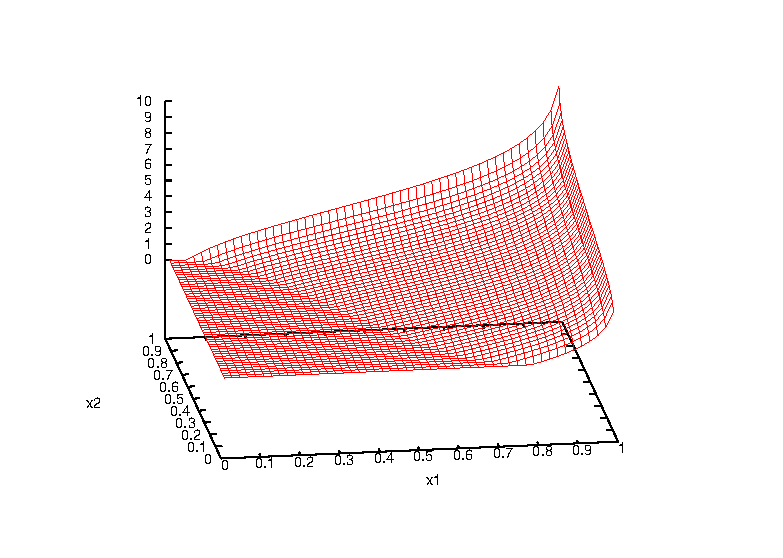
\includegraphics[width=.9\textwidth]{task5_1}
\caption{Integrand of discrete arithmetic average, $M=2,S(0)=10,r=0.1,\sigma=0.25,T=1,K=10$}
\label{fig:Task5}
\end{figure}

\section*{Task 6}
See task6.cpp for code.
\clearpage

\section*{Task 7} The first plot is a plot of the
first 100 members of the Halton sequence for $d=2$ and 100 uniform random numbers on
$(0,1)^2$ in the second plot. As we can see, the Halton sequence covers the
unit square more evenly than uniformly distributed points, i.e. "gaps" between the points are not as
big. See task7.cpp for code. \\
\begin{figure}[!ht]
\centering
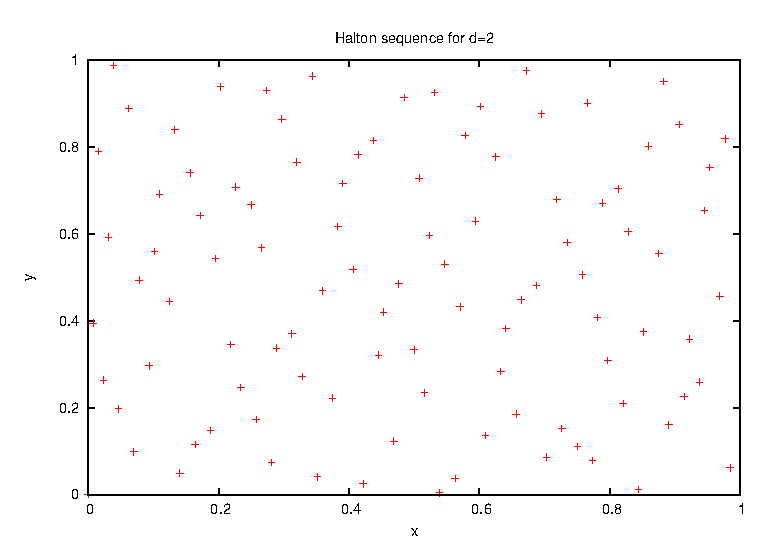
\includegraphics[width=.9\textwidth]{task7_halton.eps}
\caption{Halton sequence (2-dimensional, first 100 members)}
\label{fig:Task7a}
\end{figure}
\begin{figure}[!ht]
\centering
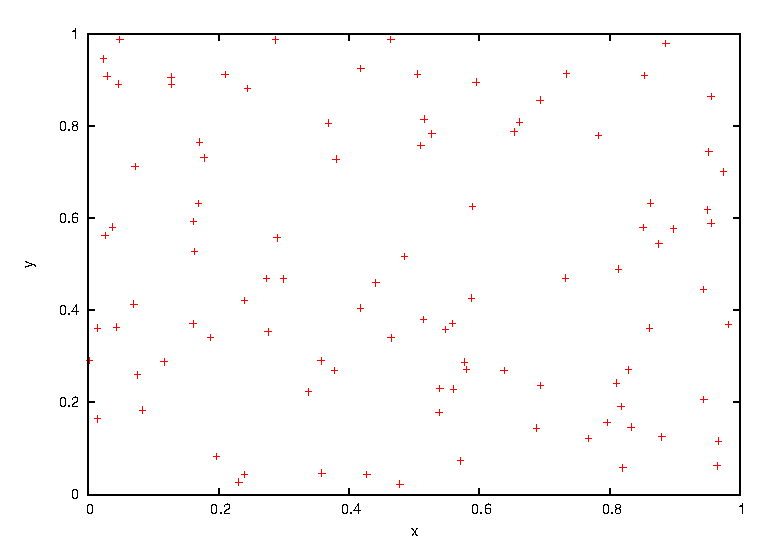
\includegraphics[width=.9\textwidth]{task7_uniform.eps}
\caption{100 uniform random numbers on $(0,1)^2$}
\label{fig:Task7b}
\end{figure}
\clearpage




\section*{Task 8}
See task8.cpp for code.

\section*{Task 9}
Nodes of different product grids.\\
\begin{figure}[!ht]
\centering
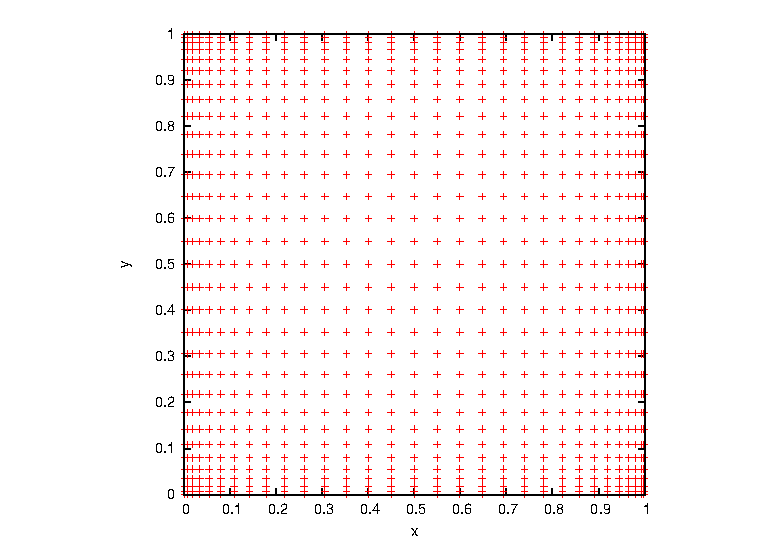
\includegraphics[width=.9\textwidth]{task9_gauss}
\caption{product rule grid for Gauss-Legendre at level 5}
\label{fig:Task9a}
\end{figure}

\begin{figure}[!ht]
\centering
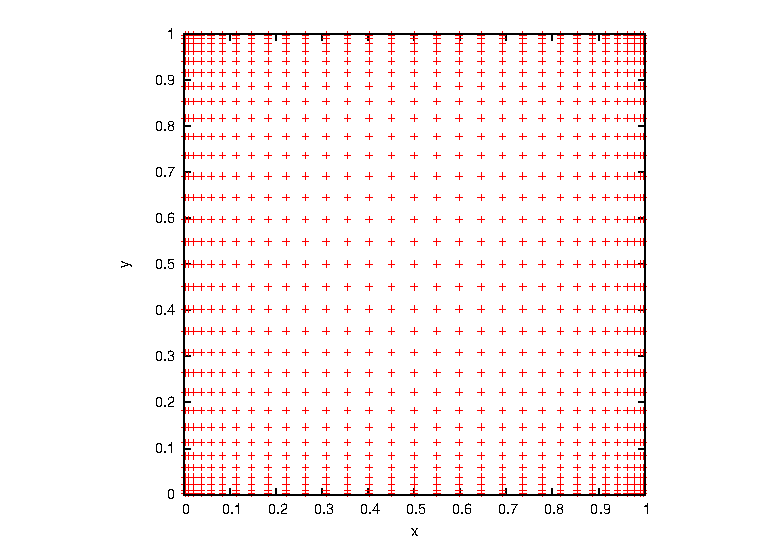
\includegraphics[width=.9\textwidth]{task9_cc}
\caption{product rule grid for Clenshaw-Curtis at level 5}
\label{fig:Task9b}
\end{figure}

\begin{figure}[!ht]
\centering
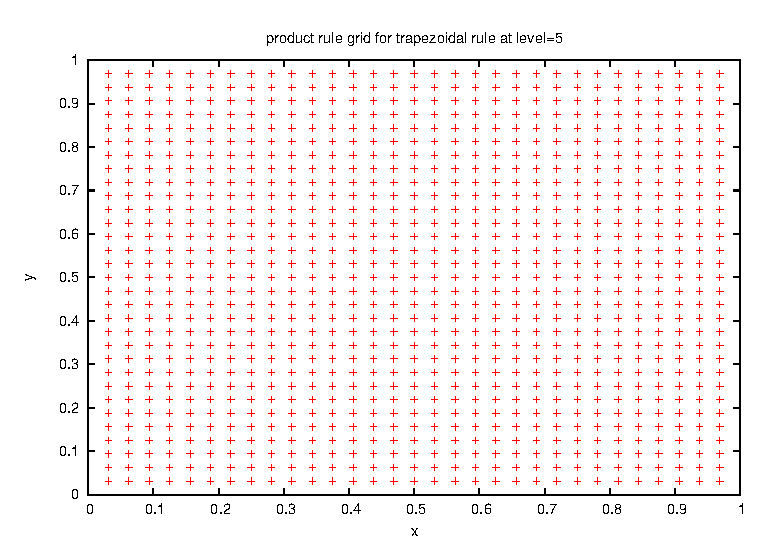
\includegraphics[width=.9\textwidth]{task9_trapezoidal}
\caption{product rule grid for trapezoidal rule at level 5}
\label{fig:Task9c}
\end{figure}
\clearpage





\section*{Task 10}
See task10.cpp for code.

\section*{Task 11}
Nodes of different sparse grids.\\
\begin{figure}[!ht]
\centering
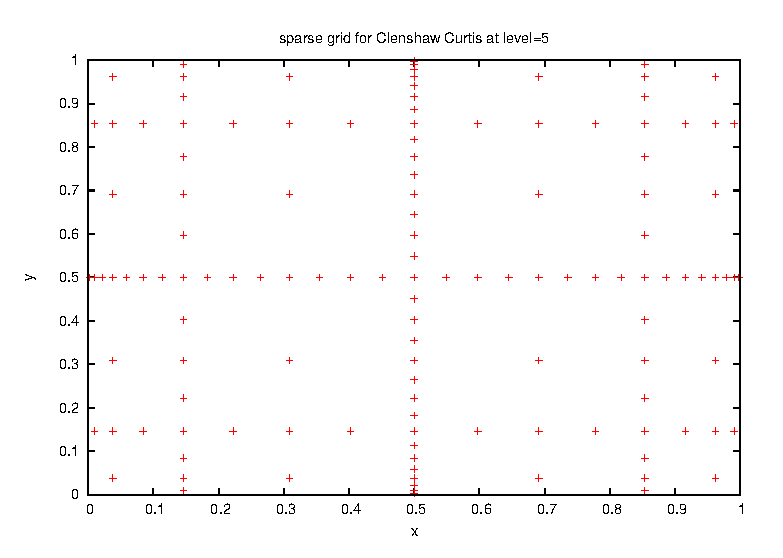
\includegraphics[width=.9\textwidth]{task11_cc5}
\caption{sparse grid for Clenshaw-Curtis at level 5}
\label{fig:Task11a}
\end{figure}

\begin{figure}[!ht]
\centering
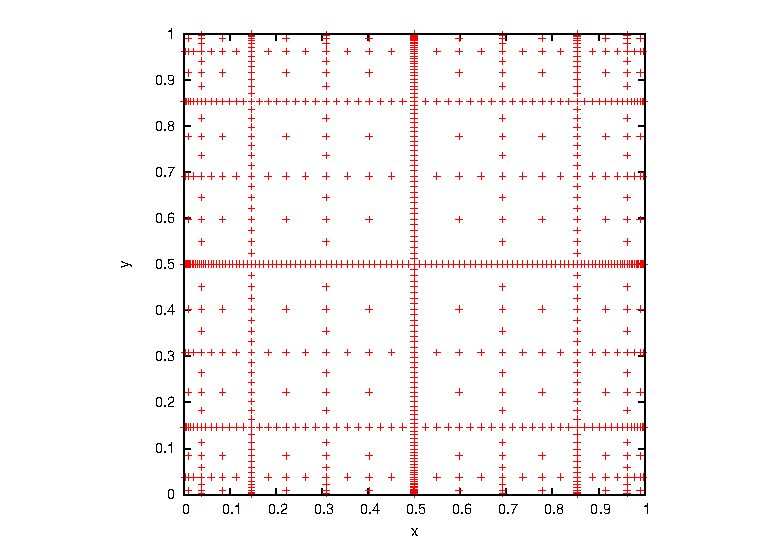
\includegraphics[width=.9\textwidth]{task11_cc7}
\caption{sparse grid for Clenshaw-Curtis at level 7}
\label{fig:Task11b}
\end{figure}

\begin{figure}[!ht]
\centering
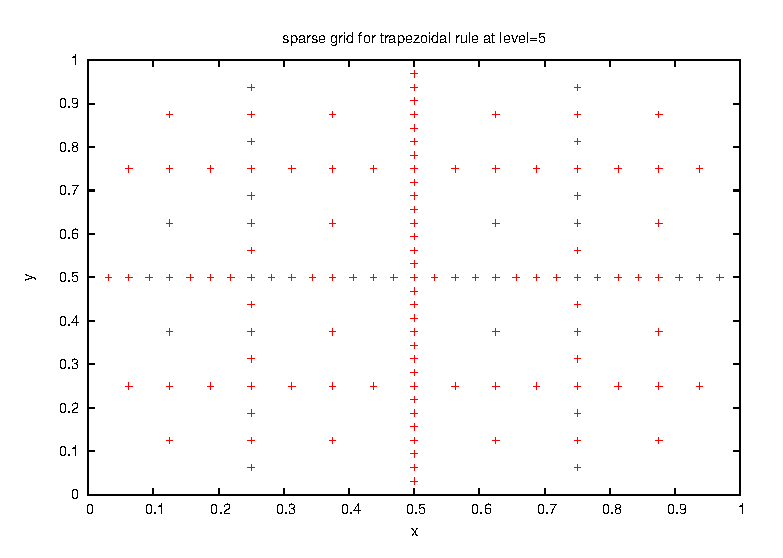
\includegraphics[width=.9\textwidth]{task11_trap_5}
\caption{sparse grid for trapezoidal rule at level 5}
\label{fig:Task11c}
\end{figure}

\begin{figure}[!ht]
\centering
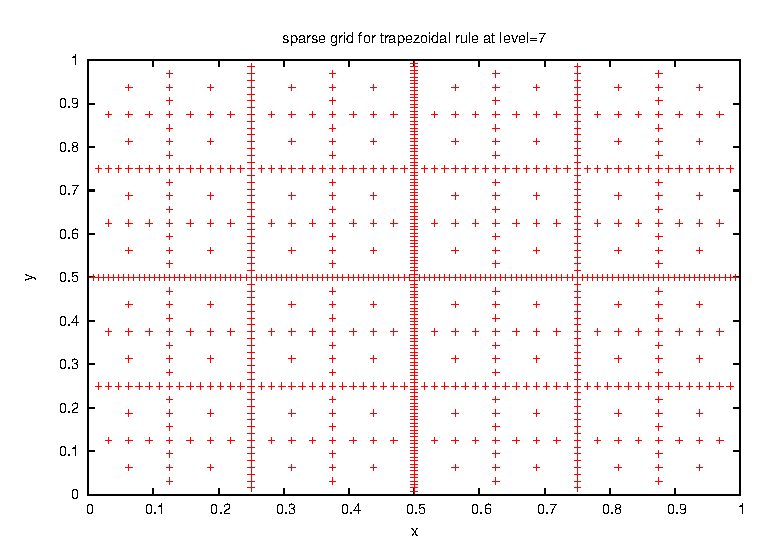
\includegraphics[width=.9\textwidth]{task11_trap_7}
\caption{sparse grid for trapezoidal rule at level 7}
\label{fig:Task11d}
\end{figure}
\clearpage





\section*{Task 12}
Comparison of product grid and sparse grid.\\
\begin{figure}[!ht]
\centering
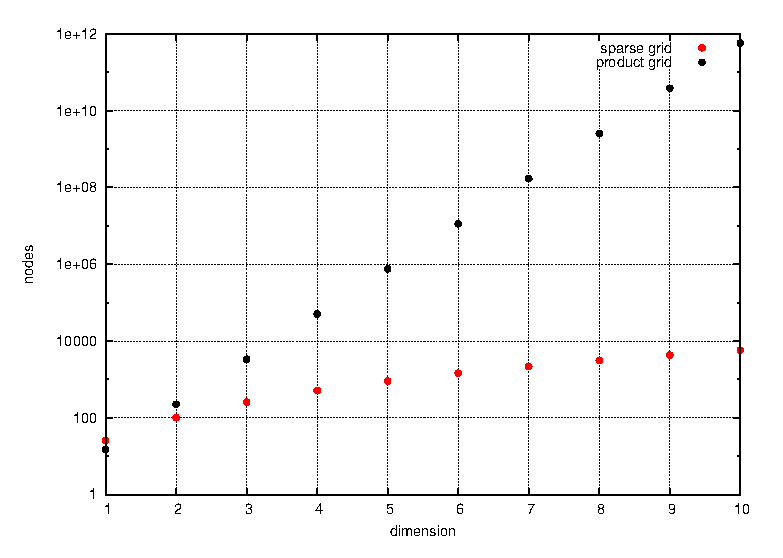
\includegraphics[width=.9\textwidth]{task12}
\caption{number of points/evaluations for sparse grid/product grid of level 4}
\label{fig:Task12}
\end{figure}
\clearpage

\section*{Task 13}
Convergence plots for integrating $f(x_1,...,x_d)=\prod_{j=1}^d (1+\gamma*\exp(x_j/2)),\gamma=0.1$.\\
\begin{figure}[!ht]
\centering
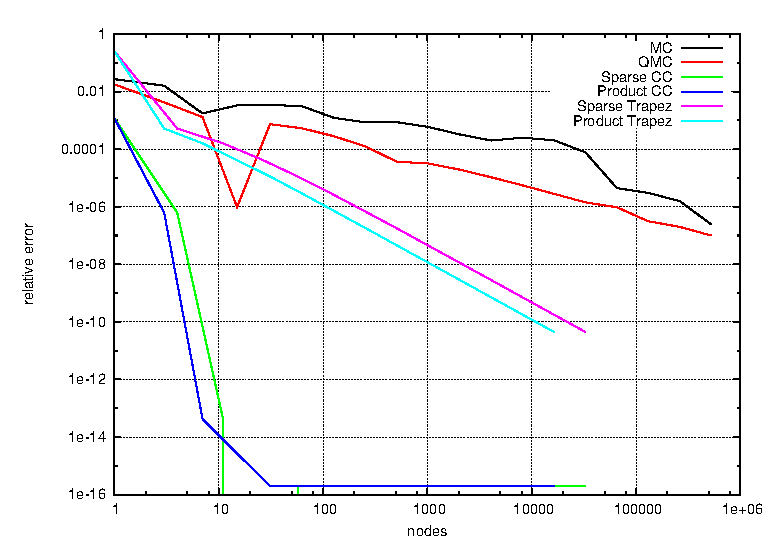
\includegraphics[width=.9\textwidth]{task13_d1}
\caption{convergence plot for $d=1$}
\label{fig:Task13a}
\end{figure}

\begin{figure}[!ht]
\centering
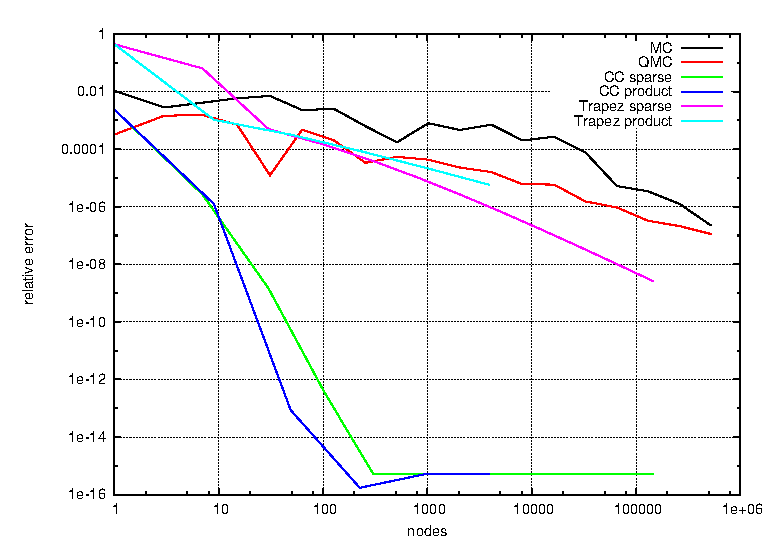
\includegraphics[width=.9\textwidth]{task13_d2}
\caption{convergence plot for $d=2$}
\label{fig:Task13b}
\end{figure}

\begin{figure}[!ht]
\centering
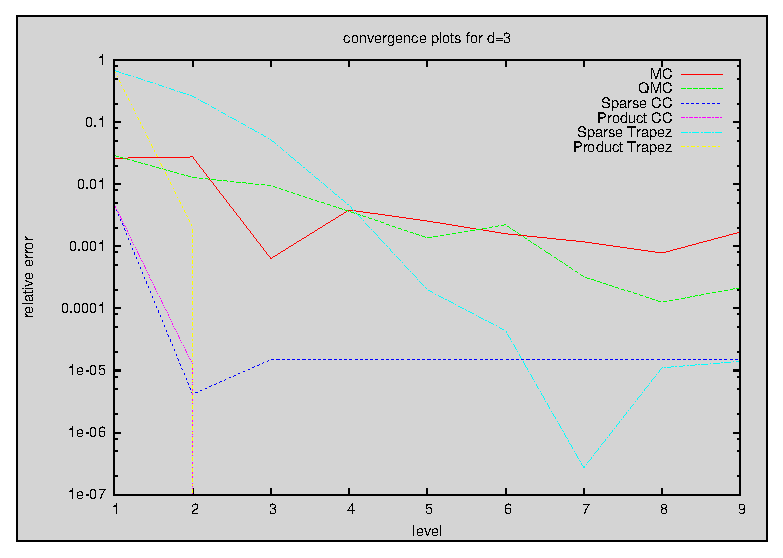
\includegraphics[width=.9\textwidth]{task13_d4}
\caption{convergence plot for $d=4$}
\label{fig:Task13c}
\end{figure}

\begin{figure}[!ht]
\centering
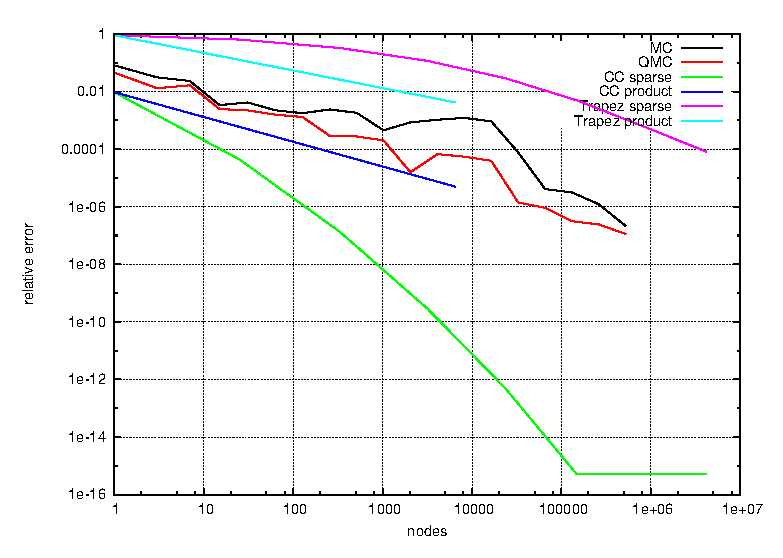
\includegraphics[width=.9\textwidth]{task13_d8}
\caption{convergence plot for $d=8$}
\label{fig:Task13d}
\end{figure}
\clearpage

\section*{Task 14}
See task14.cpp/task15.cpp

\section*{Task 15}
Integration of discrete geometric Asian option with $S(0)=10,r=0.1,\sigma=0.25,T=1,K=0,M=16$.
\begin{figure}[!ht]
\centering
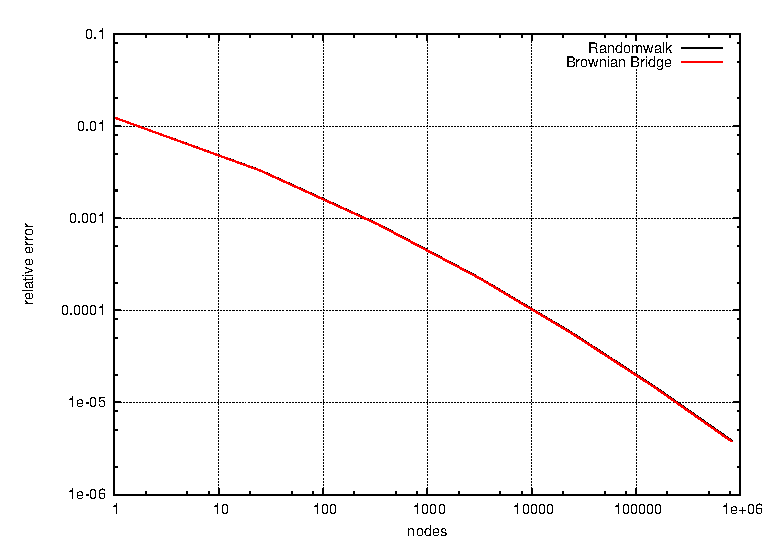
\includegraphics{task15}
\caption{Clenshaw-Curtis sparse grid}
\label{fig:Task15}
\end{figure}
\clearpage

\section*{Task 16}
Integration of discrete geometric Asian option with $S(10)=10,r=0.1,\sigma=0.25,T=1,K=0,M=8$.

\begin{figure}[!ht]
\centering
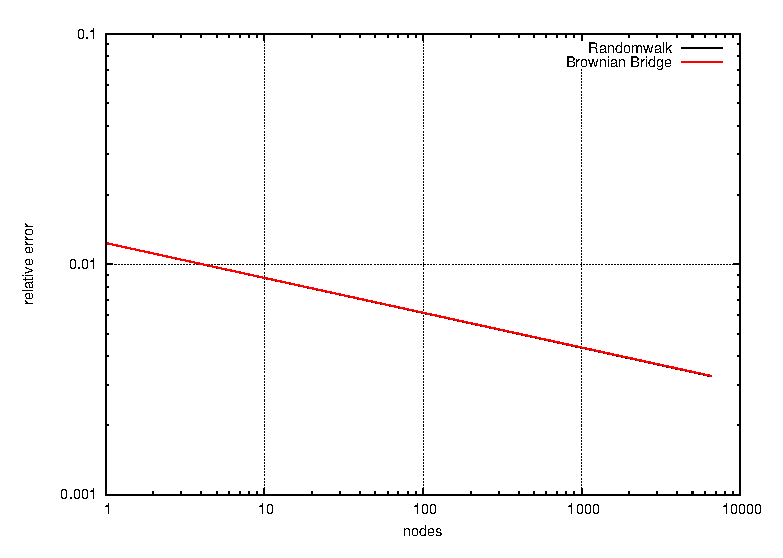
\includegraphics{task16_ccprod}
\caption{Clenshaw-Curtis Product grid}
\label{fig:Task16a}
\end{figure}

\begin{figure}[!ht]
\centering
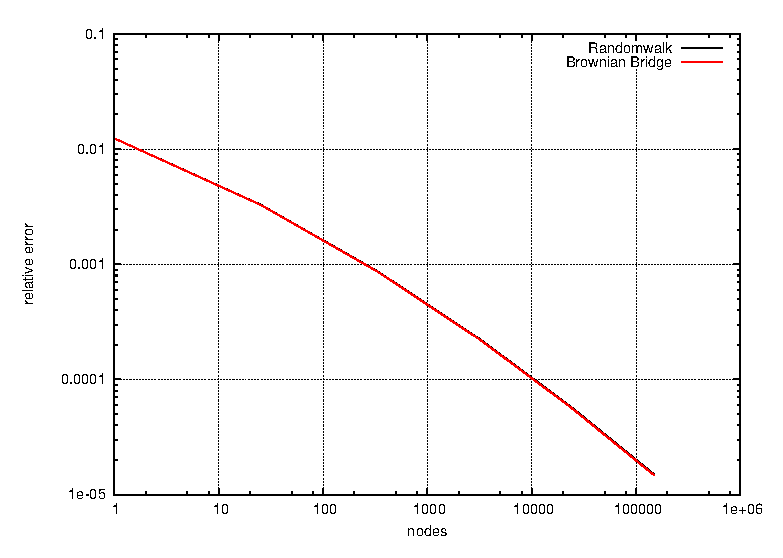
\includegraphics{task16_ccsparse}
\caption{Clenshaw-Curtis Sparse grid}
\label{fig:Task16b}
\end{figure}

\begin{figure}[!ht]
\centering
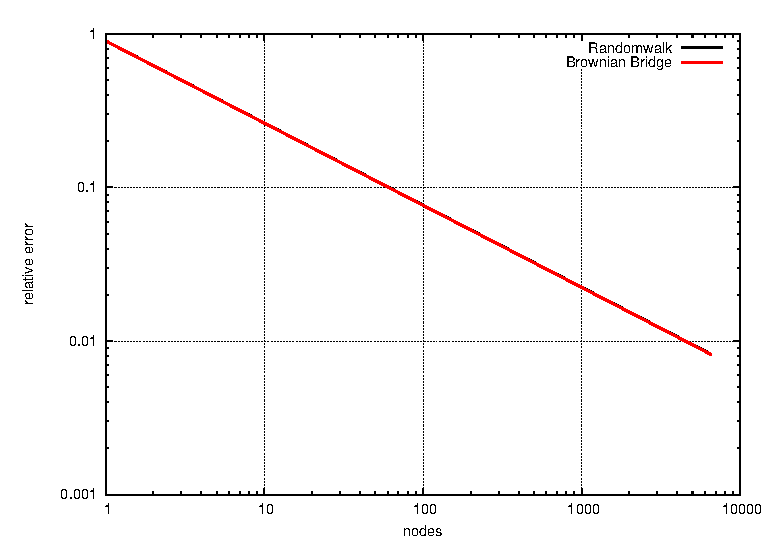
\includegraphics{task16_trapprod}
\caption{Trapezoidal rule Product grid}
\label{fig:Task16c}
\end{figure}

\begin{figure}[!ht]
\centering
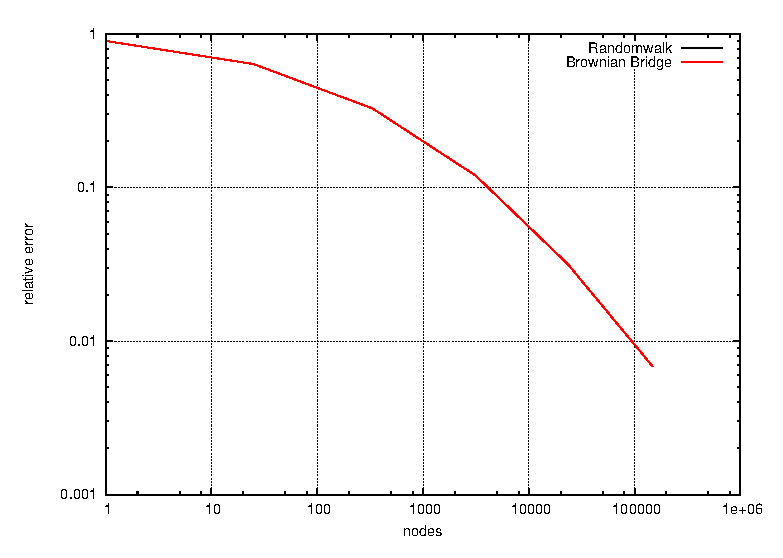
\includegraphics{task16_trapsparse}
\caption{Trapezoidal rule Sparse grid }
\label{fig:Task16d}
\end{figure}

\begin{figure}[!ht]
\centering
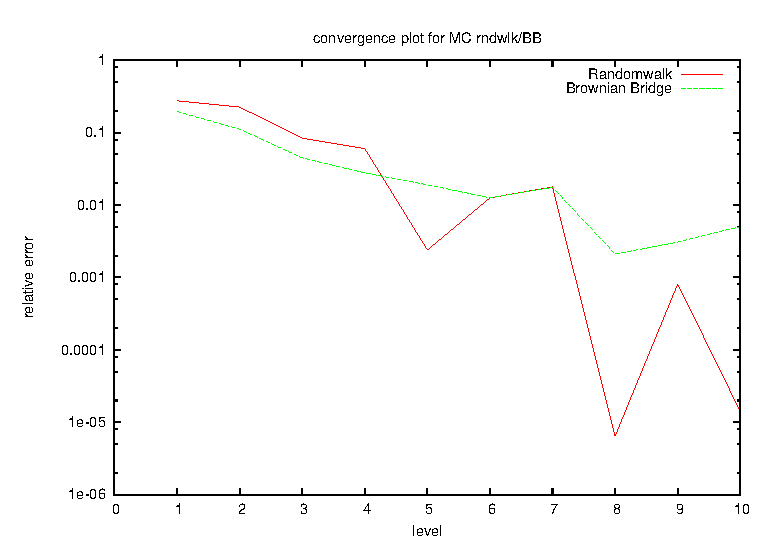
\includegraphics{task16_mc}
\caption{Monte-Carlo}
\label{fig:Task16e}
\end{figure}

\begin{figure}[!ht]
\centering
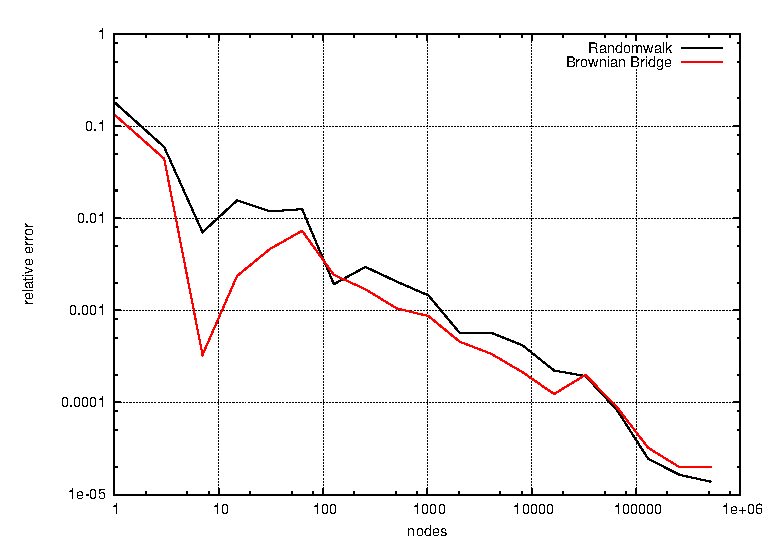
\includegraphics{task16_qmc}
\caption{Quasi-Monte-Carlo}
\label{fig:Task16f}
\end{figure}

\begin{figure}[!ht]
\centering
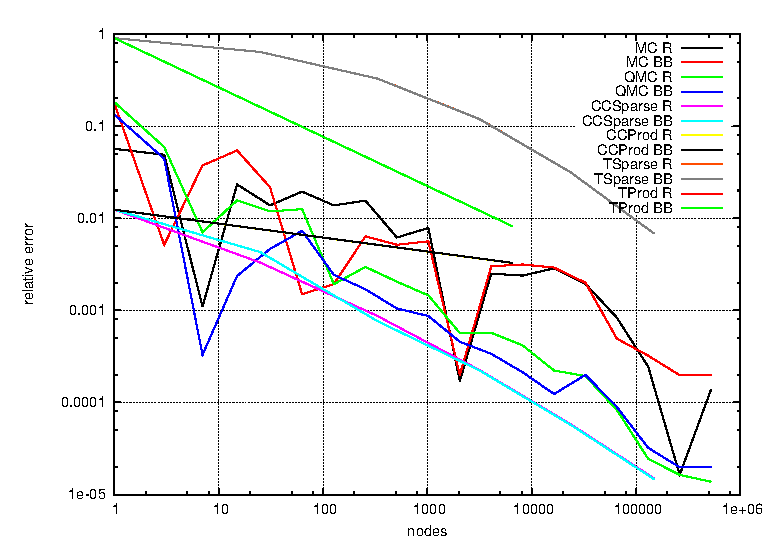
\includegraphics{task16}
\caption{All methods}
\label{fig:Task16g}
\end{figure}
\clearpage


\section*{Task 17}
Same as Task 16, but $K=10,M=64$.
\begin{figure}[!ht]
\centering
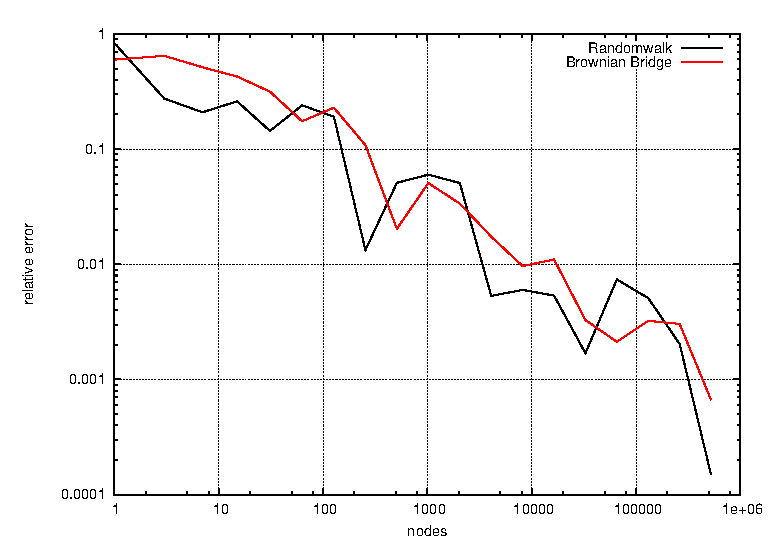
\includegraphics{task17_mc}
\caption{Monte-Carlo}
\label{fig:Task17a}
\end{figure}

\begin{figure}[!ht]
\centering
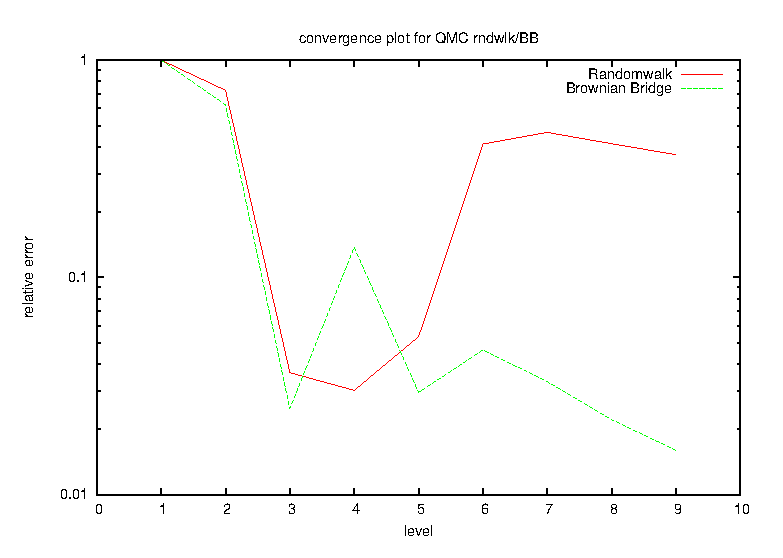
\includegraphics{task17_qmc}
\caption{Quasi-Monte-Carlo}
\label{fig:Task17b}
\end{figure}
\clearpage

\section*{Task 18} It is almost always better to not use (Q)MC, since the other
quadrature rules converge faster (even using full grids) provided the dimension is low. Clenshaw-Curtis
converges slightly faster than the Trapezoidal rule. In almost all cases sparse
grids are preferrable since they only give us a slightly worse convergence, but
a lot less points of evaluation (see Task 12). But if everything else fails, (Q)MC
works and in high dimensions, MC is better than the other methods (curse of dimension).
\end{document}
